\section{Architecture et design}

\subsection{Instrumentation}
\label{instrumentation}

Instrumenter les lignes de code exécutées n'est pas quelque chose de difficile. Il suffit simplement d'insérer une nouvelle ligne après chaque ligne existante comme représenté dans l'exemple   \ref{example_instrumentation}. Ces lignes permettront de stocker les informations relatives à l'exécution des lignes instrumentées.

\begin{figure}[h]

\begin{minipage}{.45\linewidth}

\begin{lstlisting}[linewidth=5.0cm]
maMethod :		
   instruction a
   instruction b
\end{lstlisting}

\end{minipage}
\hfill
\begin{minipage}{.45\linewidth}

\begin{lstlisting}[linewidth=11cm]
maMethod :
   instruction a
   stocker l'execution de l'instruction a
   instruction b
   stocker l'execution de l'instruction b
\end{lstlisting}

\end{minipage}


\caption{Transformation du code original vers le code instrumenté}
\label{example_instrumentation}
\end{figure}

\subsection{Interprétation}
\label{interpretation}

La couverture de ligne se calcule à l'aide de mathématiques basiques. Appelons $L_{total}$ le nombre de lignes instrumentées et $L_{exec}$ le nombre de lignes exécutées, le taux de couverture de ligne $C$ est alors le suivant :
\begin{equation}
C = { L_{exec} \over L_{total} }
\end{equation}
Cette interprétation peut être effectuée sur les classes, packages ou encore l'intégralité du projet instrumenté. Notre implémentation permet de visualiser la couverture de ligne pour les différents scopes cités.
\par C'est lors de l'instrumentation que nous allons calculer $L_{total}$. Ensuite, lors de l'exécution nous pourrons calculer dynamiquement $L_{exec}$ et donc $C$ en fonction du scope désiré.

\subsection{Design}

Notre implémentation est conçue sur le design MVC\footnote{Modèle Vue Controlleur}. Les sections suivantes ont pour but de détailler chaque partie de celui-ci.

\subsubsection{Modèle}

Le modèle de l'application contient les données nécessaires au calcul du taux de couverture. Comme expliqué dans les sections \ref{instrumentation} et \ref{interpretation}, nous avons besoin de l'ensemble des lignes de code instrumentées, ainsi que de l'ensemble des lignes de code exécutées. Le premier ensemble est construit lors de l'instrumentation, le second sera construit dynamiquement lors de l'exécution du programme instrumenté.
\newpage
\subsubsection{Vue}

La vue notifie l'utilisateur de la couverture actuelle du programme en cours d'exécution. Cette vue est dynamique, et évolue avec le temps en fonction des modifications sur le modèle.
\\
\par Nous avons mis au point deux vues :
La première est une vue textuellement qui ne permet pas la visualisation de la couverture d'une classe en particulier.
La seconde est une vue graphique qui débute à la racine du projet. Il est ensuite possible de naviguer dans le projet pour visualiser la couverture des packages ou des classes. De plus, cette vue permet pour une classe choisi d'ouvrir le fichier original en distinguant les lignes exécutées, non exécutées et non instrumentées. 

\subsubsection{Controlleur}

Le contrôleur capture les actions de utilisateur sur la vue afin de changer le scope désiré. L'utilisateur peut donc naviguer entre les différents packages ou classes du projet.

\subsection{Injection}

Lors de la phase d'instrumentation du programme, les lignes permettant de calculer $L_{exec}$ ne sont pas les seules à être insérées. Notre MVC est également injecté dans le projet pour que ce dernier puisse s'auto-instrumenter et notifier sa couverture à l'utilisateur. CoCoSpoon est uniquement utilisé pour instrumenter un programme. Il suffira ensuite de démarrer le programme exécuté pour avoir le comportement voulu. La figure \ref{workflow} représente le workflow de notre approche. 

\begin{figure}[h]
\centering
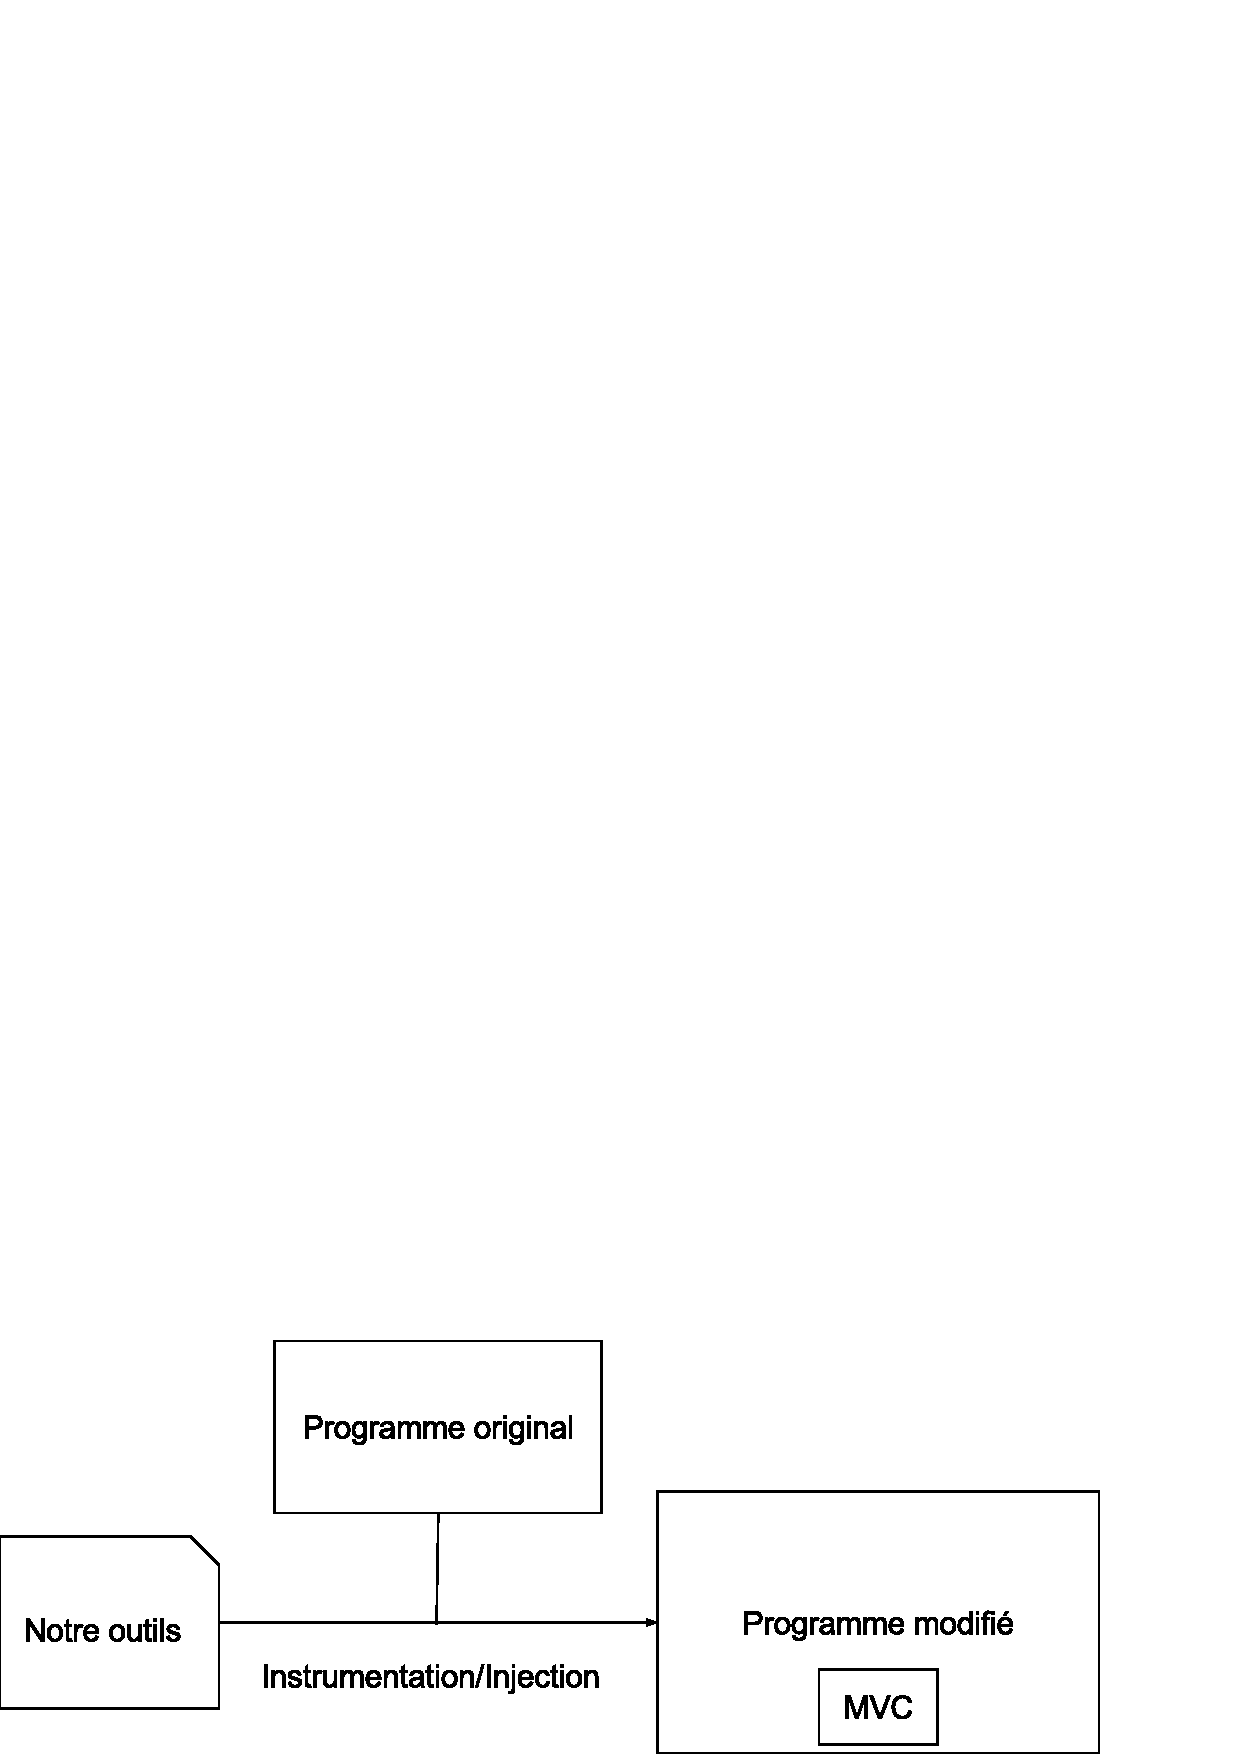
\includegraphics[scale=0.5]{workflowOPL2.png}

\caption{Workflow}
\label{workflow}
\end{figure}


